\chapter{Data presentation and analysis}
\label{chap:dataanalysis}

The prove of principle type of review was carried out on 8 from 10 planed participants. The number of participants was decreased because all information that was needed for further evaluation was already gather at this point and more test persons would not provide any new relevant data. Furthermore, the usability experiment focused more on gathering qualitative data than on quantitative data collection. Additionally, the youngest participant was three years old which deviates from the planed minimum age of two years. During the test sessions it turned out that the four and three years old participants already struggled to carry out the task which led to the conclusion that a toddler of two years of age would not have the expected understanding and motor development. The age and gender distribution of the prove of principle type of review is presented visually in table \ref{tab:participanttable}. Each participant was right handed and had no previous experience with hand-free gesture based games.


%all were right handed and novice users

\renewcommand{\arraystretch}{1.5}
 \begin{table}[h]
     \centering
     \begin{tabular}{c|c|c|c|c|c|c|c}
     \hline
        \multicolumn{1}{|l|}{\textbf{AGE:}}  &
        \multicolumn{1}{l|}{3}  &     
        \multicolumn{1}{l|}{4}  & 
        \multicolumn{1}{l|}{5}  & 
        \multicolumn{1}{l|}{7}  & 
        \multicolumn{1}{l|}{8}  & 
        \multicolumn{1}{l|}{9}  & 
        \multicolumn{1}{l|}{13} \\ \hline
        \multicolumn{1}{|l|}{\textbf{AMOUNT:}} &
        \multicolumn{1}{l|}{1}  &
        \multicolumn{1}{l|}{1}  &
        \multicolumn{1}{l|}{1}  &
        \multicolumn{1}{l|}{2}  &
        \multicolumn{1}{l|}{1}  &
        \multicolumn{1}{l|}{1}  &
        \multicolumn{1}{l|}{1}  \\ \hline
        \multicolumn{1}{|l|}{\textbf{GENDER:}}  &
        \multicolumn{1}{|l|}{F} &
        \multicolumn{1}{l|}{M}  &
        \multicolumn{1}{l|}{M}  &
        \multicolumn{1}{l|}{F/M}&
        \multicolumn{1}{l|}{F}  &
        \multicolumn{1}{l|}{M}  &
        \multicolumn{1}{l|}{F}  \\ \hline
        \multicolumn{1}{|l|}{\textbf{L/R HANDED:}} &
        \multicolumn{1}{|l|}{R} &
        \multicolumn{1}{l|}{R}  &
        \multicolumn{1}{l|}{R}  &
        \multicolumn{1}{l|}{R}  &
        \multicolumn{1}{l|}{R}  &
        \multicolumn{1}{l|}{R}  &
        \multicolumn{1}{l|}{R}  \\ \hline
        \multicolumn{1}{|l|}{\textbf{NOVICE/EXPERT:}} &
        \multicolumn{1}{|l|}{N} &
        \multicolumn{1}{l|}{N}  &
        \multicolumn{1}{l|}{N}  &
        \multicolumn{1}{l|}{N}  &
        \multicolumn{1}{l|}{N}  &
        \multicolumn{1}{l|}{N}  &
        \multicolumn{1}{l|}{N}  \\ \hline
     \end{tabular}
     \caption{Presentation of participants}
     \label{tab:participanttable}
 \end{table}
 

The age of the participant ranged from three to 13 years and included a mixture of boys and girls. 50\texttt{\%} boys and 50\texttt{\%} girls was a good balanced gender distribution. An equal distribution of gender is crucial when doing scientific research, since both genders have its own distinct characteristics. The age that most frequently appeared (mode) in this sample is 7. The arithmetic average age of the sample (mean) is also 7 and the standard deviation of the sample is 2,96 (Table \ref{tab:agestatistic}).
%Regarding the age distribution, table  \ref{tab:agestatistic} presents a statistical calculation for age distribution of the sample in this study. 
%It shows that the average age of the sample (mean) is 7 and the standard deviation of the sample is 2,96.
Additionally, the statistical calculation revealed that 87,5 \texttt{\%} of the participant finished the game at the first attempt which indicates that the game was challenging but not impossible (Figure \ref{fig:finishedgame}). 


\renewcommand{\arraystretch}{1.5}

\begin{table}[!ht]
    \centering
    \begin{tabular}{c|c|c|c}
    \hline
        \multicolumn{1}{|c|}{MEAN} &
        \multicolumn{1}{c|}{MEDIAN} &
        \multicolumn{1}{c|}{MODE} &
        \multicolumn{1}{c|}{STANDARD DEVIATION}\\ \hline
       \multicolumn{1}{|c|}{7} &
        \multicolumn{1}{c|}{7} &
        \multicolumn{1}{c|}{7} &
        \multicolumn{1}{c|}{2,96} \\ \hline
    \end{tabular}
    \caption{Average age of participants}
    \label{tab:agestatistic}
\end{table}


\begin{figure}[!ht]
   \centering
    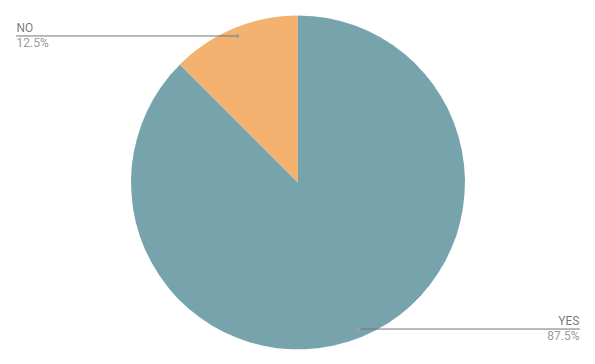
\includegraphics[width=.4\textwidth]{figures/finishedgame.png}
    \caption{Percentage of children who finished the game}
    \label{fig:finishedgame}
\end{figure}

\newpage


\section{Ability test data and questionnaire}
The primary parameters in the ability test are \textit{time} and \textit{hits} (precision) where time is in relation to hits. The less time needed to finished the game and the more precise navigation of the mole figure the better.
The closed-end questionnaire was scaled with good-ok-bad and easy-ok-hard. This scale was converted into digits where good/easy represents number 1, ok represents number 2 and bad/hard represents number 3 (Table \ref{tab:closedendedquestions}).
Sometimes, a participant did not want to answer the question (NA) or did not know (NK) the answer of a question. Since this study is based on voluntary and all compulsion could bias the outcome, the children were never force to respond to a question if they did not want to.

By inspecting the data as a whole, a global relation between entity could so be illustrated. The investigation of the relation between time and age group by using SPSS, a software for statistical analysis and data management, revealed a connection between age and finishing time. The participants were divided into three groups in order to ensure a better visual presentation of the outcome. Group one included participants from age three to age five, group two included participants from age seven to age eight, and participant from age nine to age 13 were placed in group 3.

The analyzed age-time data showed that group three had the best result in regard to the time score. They finished the task in the shortest time. 
Players in group one needed the longest time to finish the game which can be explained by their least developed motor skills. Due to the fact that the finish-time decreases with age, it suggest a relation between age and improved eye-hand coordination and increased fine motor performance (Figure \ref{fig:relationTimeAge}).

Two of the participants had a lot of hit-points at their last attempt which implies an inpatient behavior and the desire to finish the game as fast as possible. On the other hand, two other participants did improve both time and precision at the last attempt. Again, this could be explained by the child's personality and the willingness to do best. However, increased performance can also be a result of a learning effect.

Moreover, participants \texttt{\#}3, \texttt{\#}6 pointed out that the task and stabilizing of the hand was most difficult. According to the data from table \ref{tab:closedendedquestions} the older participants did not have any difficulties or experienced any fatigue regarding the midair hand position when playing the game. Furthermore, none of them had strong opinions on the difficulty level of the task, they found it manageable. The result implies a relation between age and midair hand positing. The older the participant the easier midair hand position and the execution of free-hand tasks (Figure \ref{fig:Q1}, \ref{fig:Q3}, \ref{fig:Q4}). 


Participants \texttt{\#}2, \texttt{\#}4 and \texttt{\#}5 replied to the closed-end questions (Table \ref{tab:closedendedquestions}) \textit{"safely"}. They did not have any strong opinions regarding difficulty level or affinity for the game. However, the open-ended questions (Table \ref{tab:openendedquestion}) revealed some more details and impressions. The biggest challenge for those children was to navigate the pointer and to stay in the allowed area.  

Moreover, participant \texttt{\#} 7 executed only two of three attempts. It seemed that he got bored when he found out that the game just was a prototype and that he could cheat the system, something he also pointed out in the follow up questions and conversation. (The values of his second attempt is a result of going directly from start to finish.)


An interestingly statement was made by participants \texttt{\#}1, \texttt{\#}5. They pointed out that not to touch the screen in order to control the game was problematic. This could be explained due to the unfamiliarity of touch-less navigation.

Regarding the game design and enjoyment, the participants revealed a great sympathy for the game (Figure \ref{fig:Q5}).
To the question what they like the most about the game, they pointed out the mole figure.

The result of participant \texttt{\#}3 and \texttt{\#}8 confirmed that touch-less gesture based interactions need certain motor skills, conceptual and spatial understanding of the touch-free concept (Figure \ref{fig:agegroup1}).The ability test demonstrated that these skills are not ensured in children younger than 4.

\section{Observational data}
During the ability test, the children were closely observed in order to gather information about how they handled the situation, expressed their feelings and coped with the game. Furthermore, some kids are not able to express themselves in words or get stressed when they have to replay a question. For that reason an observation could provide additional information.
There were observed several interesting issues relating to the touch-less concept. The youngest participants had too small fingers which gave them a big disadvantage when playing the game because the sensor did not recognized the stretched finger pose. They belonged to the group (\textit{group 1}) who at least understood the touch-less concept. They wanted to touched the screen in order to move the pointer or the mole. 
Most of the children were very curious about the Leap Motion sensor. They called it "the thing" because they never had seen something like that before. However, almost all of them were very eager to try the game. Especially the boys liked the idea of playing a touch-less game.
Unfortunately, not every child was patient enough. One participant was observed waving her hands and impatiently trying to make the pointer move to the mole. She also supported the pointing hand with her other hand, not because it was tiring to hold the hand above the device but rather as a help to navigate the finger in the right direction.  
Furthermore, the observation revealed that the most difficult gesture action during the sessions was the poking gesture. The game demanded a poking action in order to activate the walking mole.
Moreover, some users were very concentrated and focused on doing the task right. However they forgot about the right gesture, namely the poking finger. The finger needed to be completely stretched so the sensor could recognize the gesture. The consequence of the relaxed finger was that the system had trouble to distinguish the gesture.

Unfortunately, the prototype had some technical issues. The kids found out that it was possible to fool the system by directly going from start to finished without following the tunnel. Some other issues regarding time, hits and movement were observed as well. 


\begin{figure}[!ht]
    \centering
    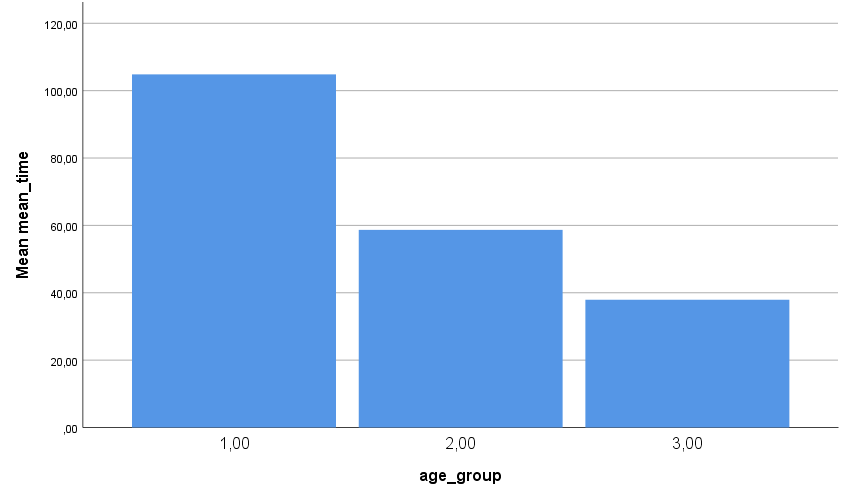
\includegraphics[width=.6\textwidth]{figures/relationTimeAge.png}
    \caption{Relation between age and time}
    \label{fig:relationTimeAge}
\end{figure}

\begin{figure}[!ht]
    \centering
    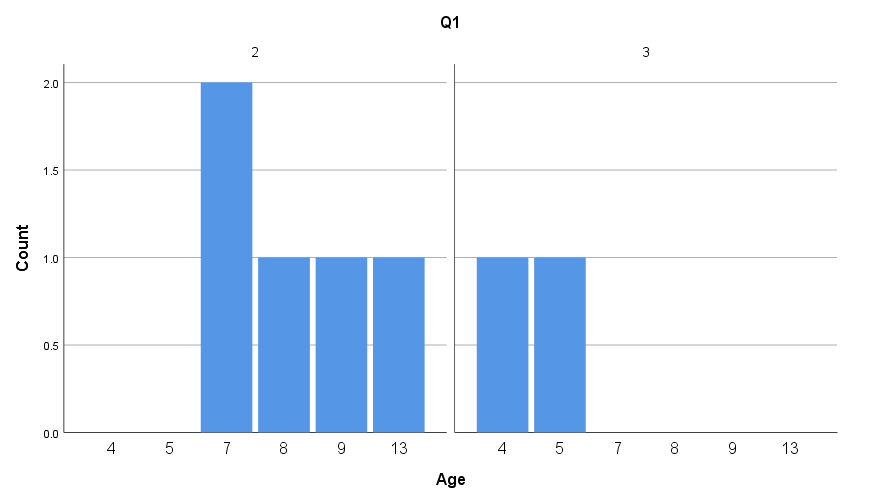
\includegraphics[width=.6\textwidth]{figures/Q1.png}
    \caption{Graphical presentation of question 1: Task difficulty}
    \label{fig:Q1}
\end{figure}
\begin{figure}[!ht]
    \centering
    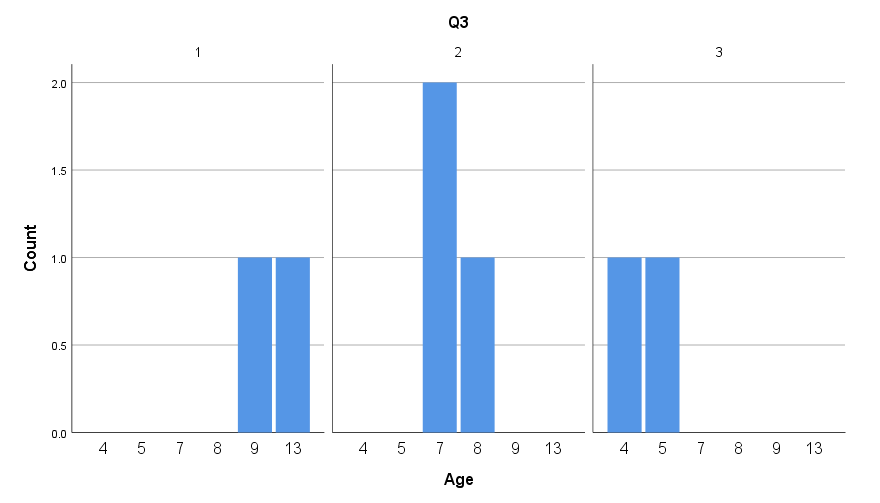
\includegraphics[width=.6\textwidth]{figures/Q3.png}
    \caption{Graphical presentation of question 3: Hand stabilization difficulty}
    \label{fig:Q3}
\end{figure}
\begin{figure}[!ht]
    \centering
    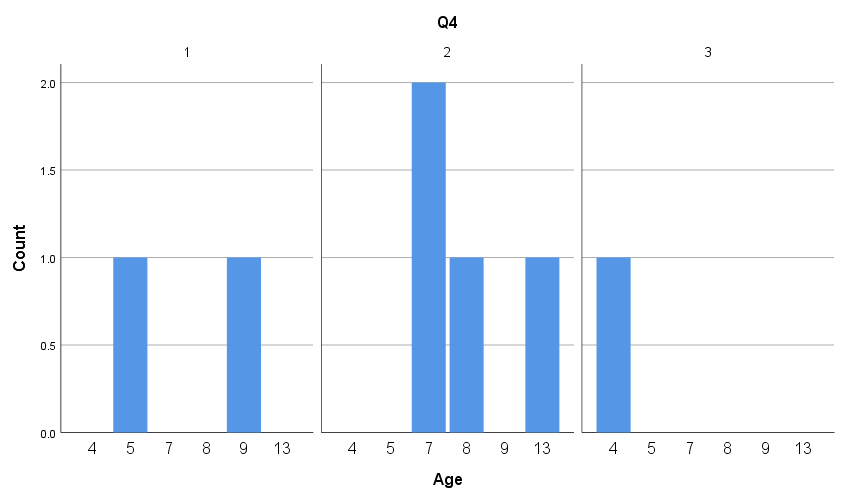
\includegraphics[width=.6\textwidth]{figures/Q4.png}
    \caption{Graphical presentation of question 4: Gesture and navigation difficulty}
    \label{fig:Q4}
\end{figure}
\begin{figure}[!ht]
    \centering
    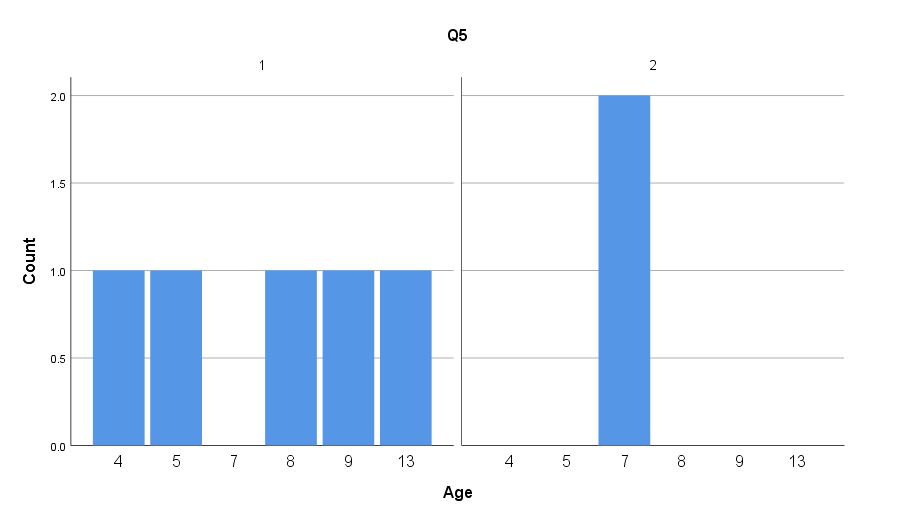
\includegraphics[width=.6\textwidth]{figures/Q5.png}
    \caption{Graphical presentation of question 5: Game sympathy }
    \label{fig:Q5}
\end{figure}



\begin{table}[!ht]
    \centering
    \begin{tabular}{c|c|c|c|c}
    \hline
    \multicolumn{1}{|c|}{\textbf{Question/participant}} &
    \multicolumn{1}{c|}{\textbf{Q1}} &
    \multicolumn{1}{c|}{\textbf{Q3}} &
    \multicolumn{1}{c|}{\textbf{Q4}} &
    \multicolumn{1}{c|}{\textbf{Q5}} \\ \hline
 
    \multicolumn{1}{|c|}{\textbf{P\texttt{\#}3}} &
    \multicolumn{1}{c|}{3} &
    \multicolumn{1}{c|}{3} &
    \multicolumn{1}{c|}{3} &
    \multicolumn{1}{c|}{1} \\ \hline
    \multicolumn{1}{|c|}{\textbf{P\texttt{\#}6}} &
    \multicolumn{1}{c|}{3} &
    \multicolumn{1}{c|}{3} &
    \multicolumn{1}{c|}{1} &
    \multicolumn{1}{c|}{1} \\ \hline
    \multicolumn{1}{|c|}{\textbf{P\texttt{\#}8}} &
    \multicolumn{1}{c|}{-} &
    \multicolumn{1}{c|}{-} &
    \multicolumn{1}{c|}{-} &
    \multicolumn{1}{c|}{-} \\ \hline
    \multicolumn{1}{|c|}{\textbf{P\texttt{\#}2}} &
    \multicolumn{1}{c|}{2} &
    \multicolumn{1}{c|}{2} &
    \multicolumn{1}{c|}{2} &
    \multicolumn{1}{c|}{1} \\ \hline
    \multicolumn{1}{|c|}{\textbf{P\texttt{\#}4}} &
    \multicolumn{1}{c|}{2} &
    \multicolumn{1}{c|}{2} &
    \multicolumn{1}{c|}{2} &
    \multicolumn{1}{c|}{2} \\ \hline
    \multicolumn{1}{|c|}{\textbf{P\texttt{\#}5}} &
    \multicolumn{1}{c|}{2} &
    \multicolumn{1}{c|}{2} &
    \multicolumn{1}{c|}{2} &
    \multicolumn{1}{c|}{2} \\ \hline
    \multicolumn{1}{|c|}{\textbf{P\texttt{\#}1}} &
    \multicolumn{1}{c|}{2} &
    \multicolumn{1}{c|}{1} &
    \multicolumn{1}{c|}{2} &
    \multicolumn{1}{c|}{1} \\ \hline
    \multicolumn{1}{|c|}{\textbf{P\texttt{\#}7}} &
    \multicolumn{1}{c|}{2} &
    \multicolumn{1}{c|}{1} &
    \multicolumn{1}{c|}{1} &
    \multicolumn{1}{c|}{2} \\ \hline
    \end{tabular}
    \caption{Closed-ended questions}
    \label{tab:closedendedquestions}
\end{table}


\begin{table}[!ht]
    \centering
    \begin{tabular}{c|c|c|c|c}
    \hline
  %  \rowcolor{1}{green}
    \multicolumn{1}{|c|}{\textbf{Question/participant}} &
    \multicolumn{1}{c|}{\textbf{Q2}} &
    \multicolumn{1}{c|}{\textbf{Q6}} &
    \multicolumn{1}{c|}{\textbf{Q7}} &
    \multicolumn{1}{c|}{\textbf{Q8}} \\ \hline
    \multicolumn{1}{|c|}{\textbf{P\texttt{\#}3}} &
    \multicolumn{1}{c|}{NK} &
    \multicolumn{1}{c|}{mole} &
    \multicolumn{1}{c|}{NA} &
    \multicolumn{1}{c|}{NA} \\ \hline
    \multicolumn{1}{|c|}{\textbf{P\texttt{\#}6}} &
    \multicolumn{1}{c|}{NA} &
    \multicolumn{1}{c|}{mole} &
    \multicolumn{1}{c|}{navigate - pointer} &
    \multicolumn{1}{c|}{OK} \\ \hline
    \multicolumn{1}{|c|}{\textbf{P\texttt{\#}8}} &
    \multicolumn{1}{c|}{-} &
    \multicolumn{1}{c|}{-} &
    \multicolumn{1}{c|}{-} &
    \multicolumn{1}{c|}{-} \\ \hline
        \multicolumn{1}{|c|}{\textbf{P\texttt{\#}2}} &
    \multicolumn{1}{c|}{not to cross the line} &
    \multicolumn{1}{c|}{NA} &
    \multicolumn{1}{c|}{NA} &
    \multicolumn{1}{c|}{OK} \\ \hline
    \multicolumn{1}{|c|}{\textbf{P\texttt{\#}4}} &
    \multicolumn{1}{c|}{to move the pointer} &
    \multicolumn{1}{c|}{follow the white path} &
    \multicolumn{1}{c|}{navigate - pointer} &
    \multicolumn{1}{c|}{OK} \\ \hline
    \multicolumn{1}{|c|}{\textbf{P\texttt{\#}5}} &
    \multicolumn{1}{c|}{not to touch the screen} &
    \multicolumn{1}{c|}{NA} &
    \multicolumn{1}{c|}{NA} &
    \multicolumn{1}{c|}{OK} \\ \hline
       \multicolumn{1}{|c|}{\textbf{P\texttt{\#}1}} &
    \multicolumn{1}{c|}{not to touch the screen} &
    \multicolumn{1}{c|}{NA} &
    \multicolumn{1}{c|}{NA} &
    \multicolumn{1}{c|}{OK} \\ \hline
    \multicolumn{1}{|c|}{\textbf{P\texttt{\#}7}} &
    \multicolumn{1}{c|}{stay in tunnel} &
    \multicolumn{1}{c|}{challenging} &
    \multicolumn{1}{c|}{uncontrolled mole} &
    \multicolumn{1}{c|}{OK} \\ \hline
    \end{tabular}
    \caption{Open-ended questions}
    \label{tab:openendedquestion}
\end{table}





\begin{figure}[!ht]

    \centering
    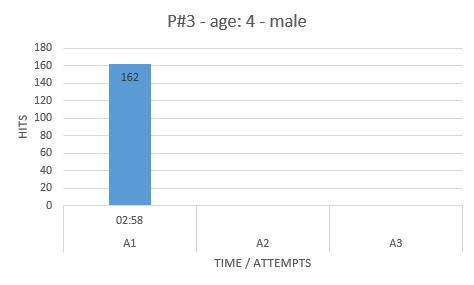
\includegraphics[width=.6\textwidth]{figures/p3.png}
   %  \caption{Participant \texttt{\#}3}
    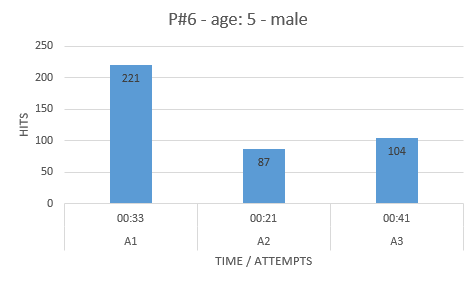
\includegraphics[width=.6\textwidth]{figures/p6.png}
 %   \caption{Participant \texttt{\#}6}
        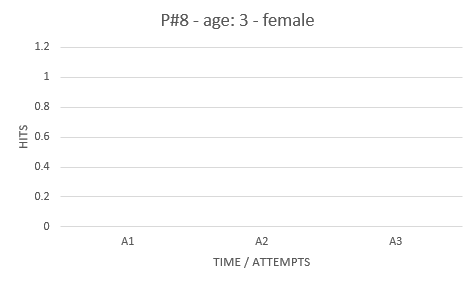
\includegraphics[width=.6\textwidth]{figures/p8.png}
    \caption{Time/hit parameters. Data presentation of group 1. Participants \texttt{\#}3, 6 and 8}
    \label{fig:agegroup1}
\end{figure}

\begin{figure}[!ht]
    \centering
    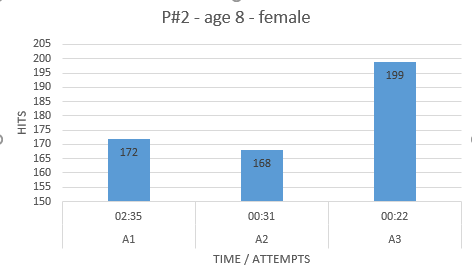
\includegraphics[width=.6\textwidth]{figures/p2.png}
    % \caption{Participant \texttt{\#}2}
    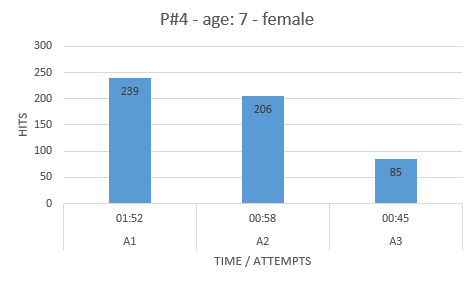
\includegraphics[width=.6\textwidth]{figures/p4.png}
   % \caption{Participant \texttt{\#}4}
        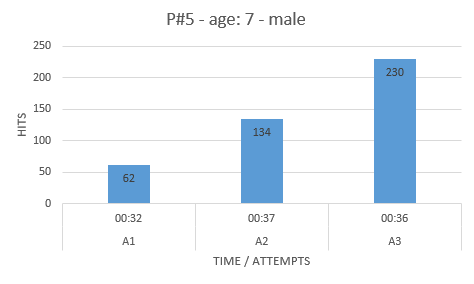
\includegraphics[width=.6\textwidth]{figures/p5.png}
    \caption{Time/hit parameters. Data presentation of group 2. Participants \texttt{\#}2, 4 and 5}
    \label{fig:agegroup2}
\end{figure}

\begin{figure}[!ht]
    \centering
    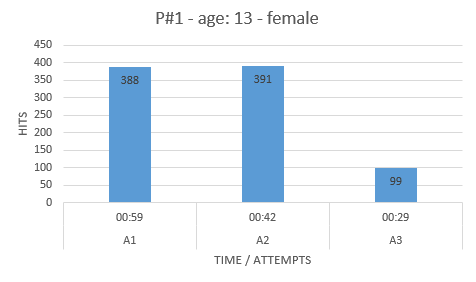
\includegraphics[width=.6\textwidth]{figures/p1.png}
     %\caption{Participant \texttt{\#}1}
    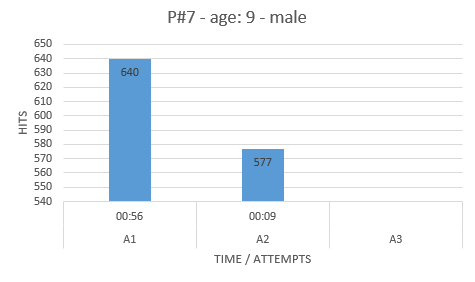
\includegraphics[width=.6\textwidth]{figures/p7.png}
    \caption{Time/hit parameters. Data presentation of group 3. Participants \texttt{\#}1 and 7}

    \label{fig:agegroup3}
\end{figure}





